\documentclass[a5paper,twoside,11pt]{report}

%%%%%%%%%% Packages %%%%%%%%%%
\usepackage[outer=2cm, inner=2cm, bottom=2.5cm, footnotesep=1cm]{geometry}
\usepackage[utf8x]{inputenc}
\usepackage[super]{nth}
\usepackage[bottom]{footmisc} 
%\usepackage[backend=biber, style=authoryear-icomp, block=ragged]{biblatex}
\usepackage{longtable}
\usepackage{fancyhdr}
\usepackage{graphicx}
\usepackage{wrapfig}
\usepackage{enumitem}
%\usepackage[utf8]{inputenc}
\usepackage{fontspec}
\usepackage[greek,english,latin]{babel} 
\usepackage{epigraph}
\usepackage{lmodern}
\usepackage{afterpage}
\usepackage{nonumonpart}
\usepackage{titlesec}
\usepackage{microtype}
\usepackage{titling} 
\usepackage[T1]{fontenc}
\usepackage{bold-extra}
\usepackage{listings}
\usepackage{xcolor}
\usepackage{libertine}
\linespread{1.1}
\usepackage[nopbinverse,nocritical,noend,noeledsec,nofamiliar,noledgroup]{reledmac}
\usepackage[]{reledpar}

\raggedbottom

\makeindex
%\setgoalfraction{2}
%\addbibresource{bibliography.bib}

% \SetWatermarkText{Preview}
\newlength\longest
\setlength{\marginparwidth}{0pt}
\setlength{\headheight}{15pt}

\titleformat{\section}[wrap]
{\normalfont\bfseries}
{\thesection.}{0.5em}{}
\titlespacing{\section}{12pc}{1.5ex plus .1ex minus .2ex}{1pc}

\definecolor{backcolor}{rgb}{0.95,0.95,0.92}

\lstdefinestyle{mystyle}{
      backgroundcolor=\color{backcolor},
      basicstyle=\ttfamily\footnotesize,
      breakatwhitespace=false,         
      breaklines=true,                 
      captionpos=b,                    
      keepspaces=true,                 
      numbers=left,                    
      numbersep=5pt,                  
      showspaces=false,                
      showstringspaces=false,
      showtabs=false,                  
      tabsize=2
}
\lstset{style=mystyle}
%%%%%%%%%% Fancy HDR %%%%%%%%%%
\pagestyle{fancy}
\fancyhf{}
\fancyhead[LE,RO]{\thepage}
\fancyhead[LO]{\nouppercase{\leftmark}}
\fancyhead[RE]{\textsc{The Apocalypse of John}}
\fancypagestyle{plain}{
\fancyhf{} 
\fancyhead[LE,RO]{\thepage}
\fancyhead[LO]{\leftmark}
\fancyhead[RE]{\textsc{The Apocalypse of John}}}

\begin{document}
\pagenumbering{gobble} 

%%%%%%%%%% Pretitle %%%%%%%%%%
\thispagestyle{empty}
\begin{center}
	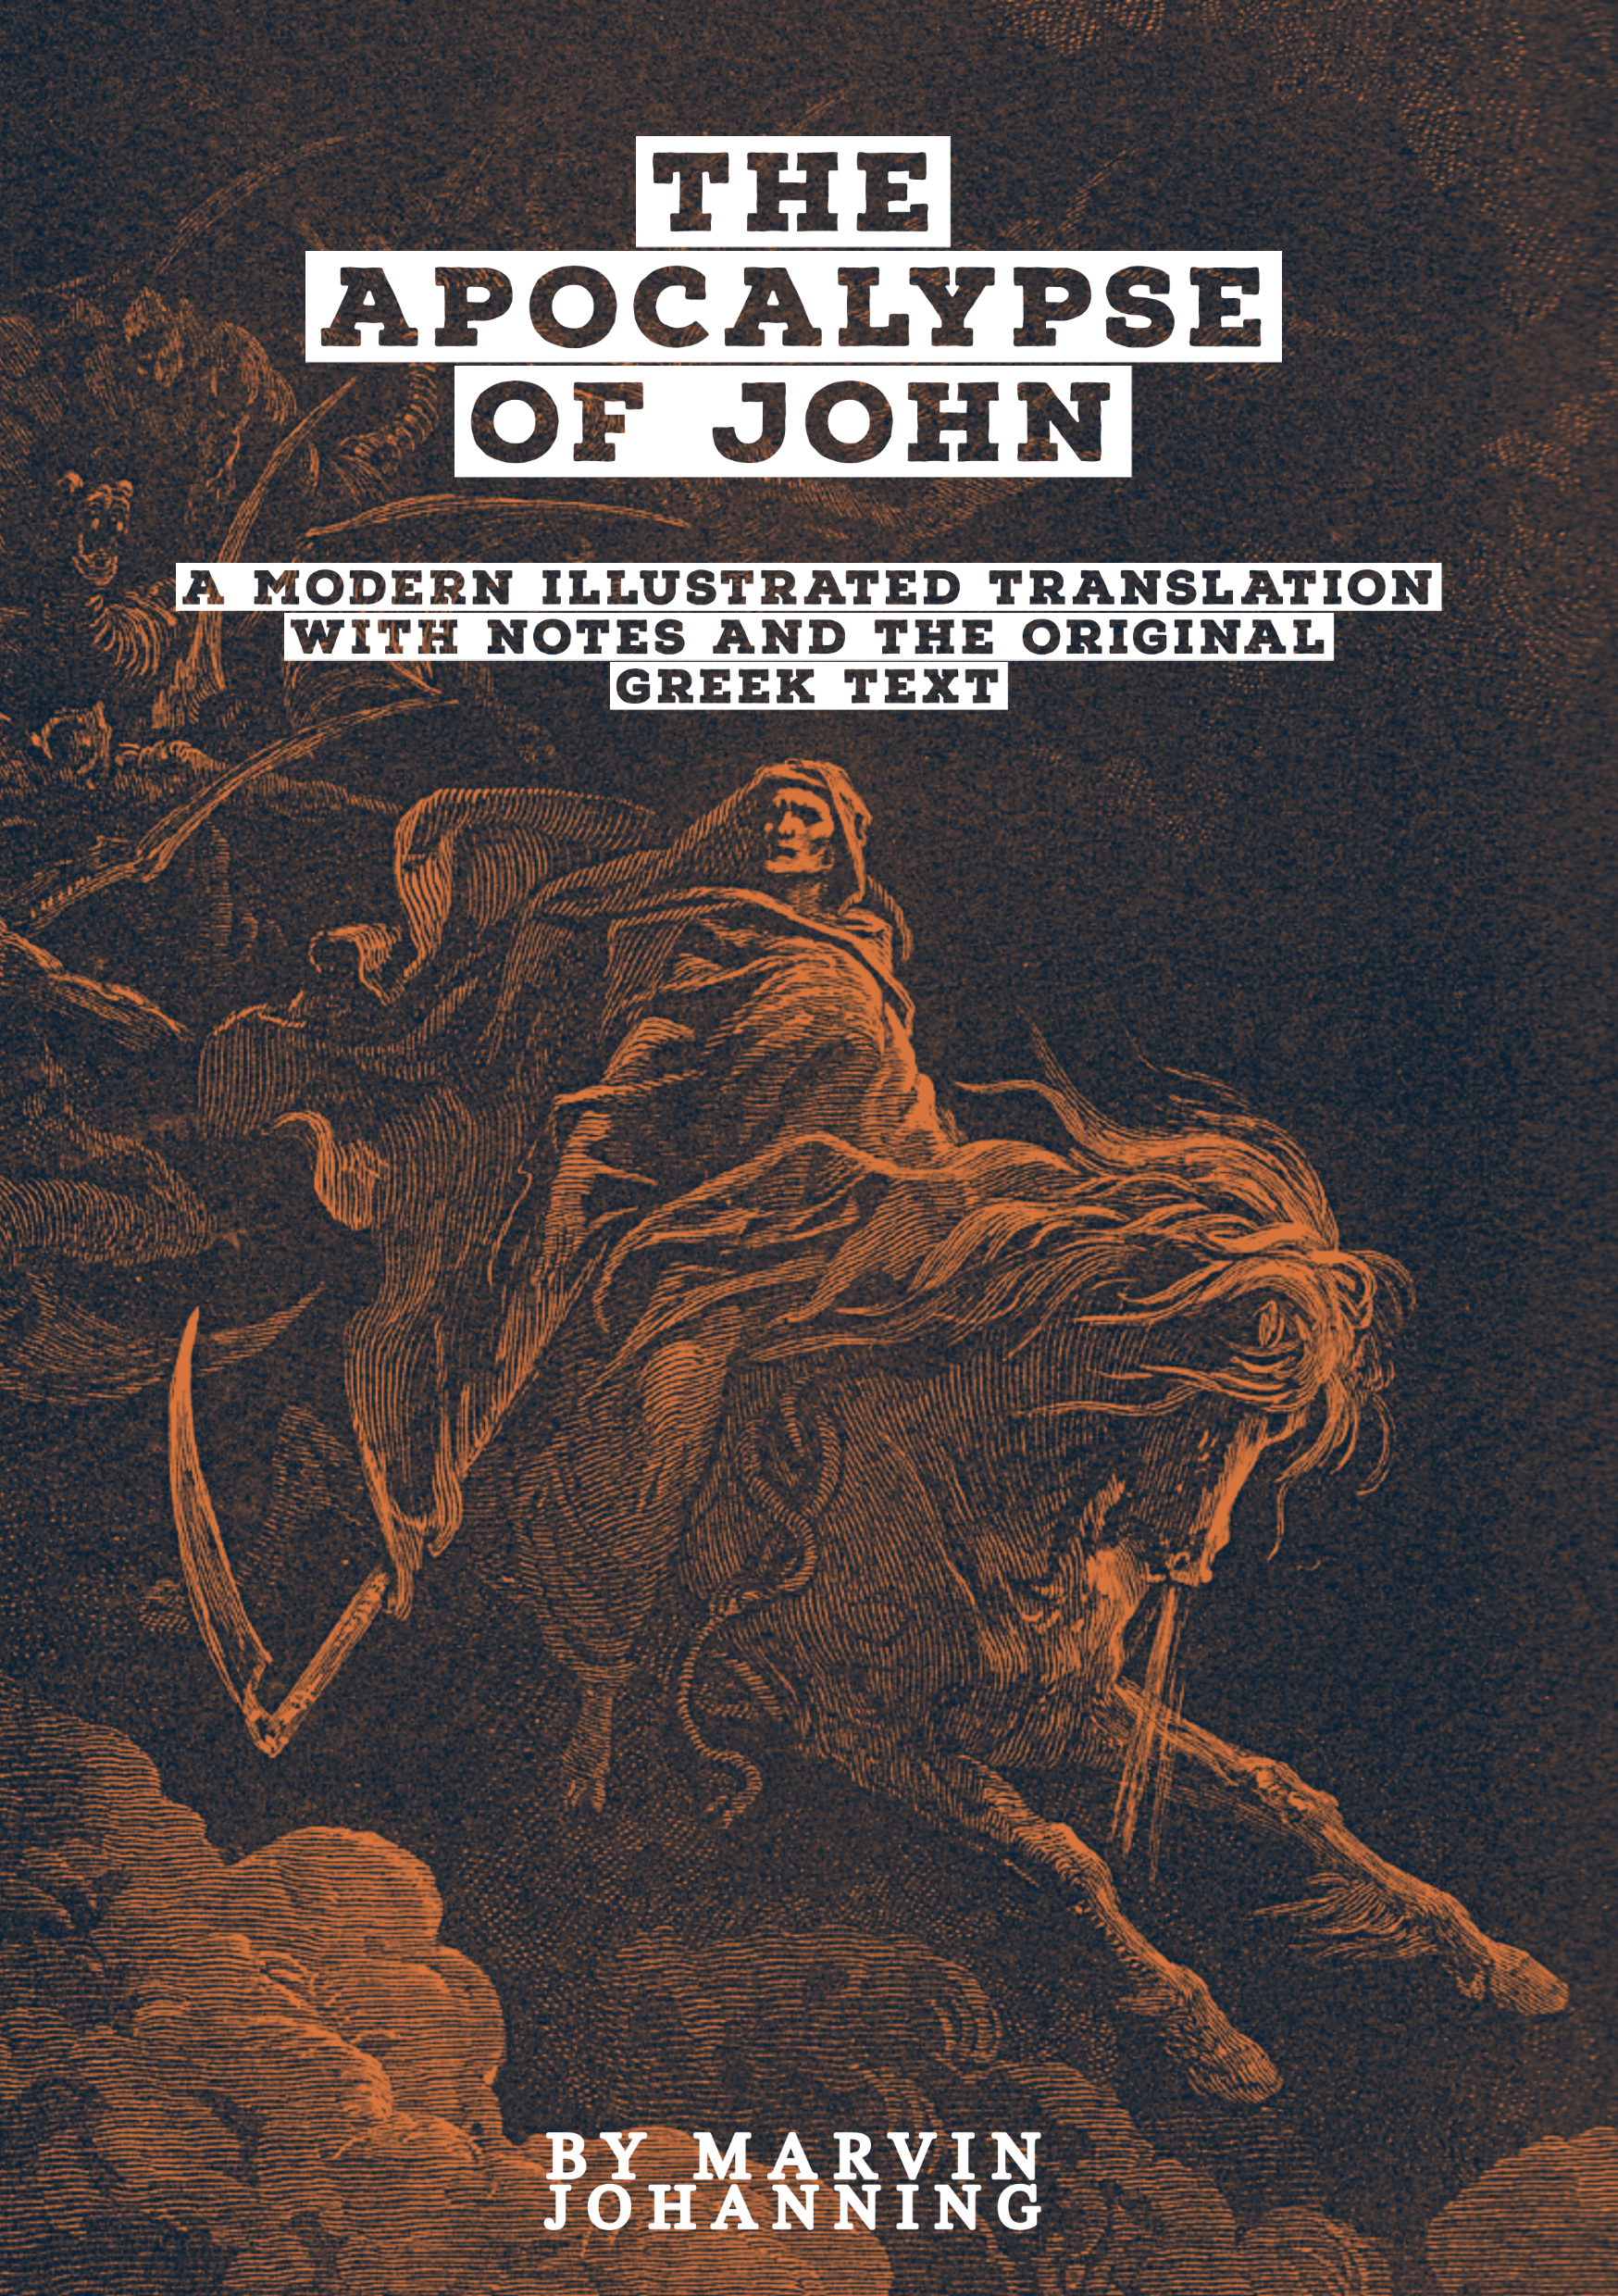
\includegraphics[scale=0.162]{images/cover.png}
\end{center}
\newpage

%%%%%%%%%% EMPTY PAGE %%%%%%%%%% 
\thispagestyle{empty}
  \mbox{}
  \newpage

%%%%%%%%%% Posttitle %%%%%%%%%% 
\title{%
  The Apocalypse of John\\
  \begin{center}
    \textit{A modern illustrated translation with notes and the original Greek text}
  \end{center}
}
\author{By Marvin Johanning}
\date{}
\maketitle

%%%%%%%%%% Copyright and Impressum %%%%%%%%%%
\thispagestyle{empty}
\noindent\textsc{\underline{Text}}: © Copyright 2021 Marvin Johanning

\noindent\textsc{\underline{Greek text}}: Eberhard Nestle's ``Novum Testamentum Graece'', 1904

\noindent\textsc{\underline{Cover design}}: © Copyright 2021 Marvin Johanning

\noindent\textsc{\underline{Cover image}}: Gustave Doré - Death on the Pale Horse, 1865

\bigskip

\noindent© 2021 by Marvin Johanning\\``The Apocalypse of John: a modern illustrated translation with notes and the original Greek text'' by Marvin Johanning is licensed under CC BY-NC-ND 4.0. To view a copy of this license, visit https://creativecom\\mons.org/licenses/by-nc-nd/4.0.\\This copyright statement does not apply for the images and illustrations found in this book; these are all in the public domain and can be used freely. 

\vspace{10mm}\noindent\textsc{Publishing}: \\
Marvin Johanning\\
Heeper Str.  214\\
33607 Bielefeld\\
info@marvinjohanning.de

\vspace{5mm}\noindent\textsc{Printing}: epubli – ein Service der neopubli GmbH, Berlin
\newpage


%%%%%%%%%% Introductory quote %%%%%%%%%%
\clearpage
\thispagestyle{empty}
\null\vfill
\settowidth\longest{\huge\itshape Καὶ εἶδον οὐρανὸν καινὸν καὶ γῆν καινήν}
\begin{center}
\parbox{\longest}{%
  \raggedright{\huge\itshape%
    Καὶ εἶδον οὐρανὸν καινὸν καὶ γῆν καινήν· ὁ γὰρ πρῶτος οὐρανὸς καὶ ἡ πρώτη γῆ παρῆλθε,  καὶ ἡ θάλασσα οὐκ ἔστιν ἔτι. \par\bigskip
  }
  \raggedleft\Large\MakeUppercase{Rev. 21:1}\par%
}
\vfill\vfill
\clearpage\newpage
\end{center}
\newpage

%%%%%%%%%% Table of Contents %%%%%%%%%%
\tableofcontents
\newpage

%%%%%%%%%% Introduction and Preface %%%%%%%%%%
%%%%%%%%%% Introduction %%%%%%%%%%
\chapter*{Introduction to this translation \\ \large On translating ancient texts}
  \markboth{Introduction to this translation}{Introduction to this translation}
  \addcontentsline{toc}{chapter}{Introduction to this translation}
  
Translations of the New Testament are plentiful — indeed, the vast majority of translations one can attain nowadays are much more professionally made and have had dozens of people working for hundreds upon hundreds of hours perfecting them. Therefore, it may come as a surprise to some that I — someone who has written what you are about to read in his free-time and who has never “professionally” studied Ancient Greek — would take it upon myself to write my own translation of one of the books of the New Testament. 

Thus, in order for you to understand why this particular translation exists and how it differs from other translations, I decided to write this introduction, detailing the philosophy behind the manner in which I translate texts.

\section*{Cultural issues}
  \addcontentsline{toc}{section}{Cultural issues}
  
 Translating texts from another language is never as straight-forward as some people might believe; one cannot simply pick up a dictionary, start translating and expect to have a coherent result thereafter. I have met a number of people who sincerely believe that they will be able to study a language by solely learning vocabulary and leaving the acquisition of grammatical concepts to ``intuition''. 
 
 Such approaches are — in my opinion — bound to fail, unless it is one's goal to part-take in a spelling contest in another language (as some people have, indeed, previously done). 
 
 Instead, translating a text requires not only an at least somewhat firm grasp of the language's grammatical concepts — and how they might be translated properly without distorting their meaning too considerably —, but also an understanding of the source text and the cultural background of the people who speak the language being translated from. 
 
 Of the above-mentioned skills, however, only two can be harnessed with relative ease, namely the attaining of a firm understanding of the grammatical concepts of the language and of the text being translated; the latter skill — (somewhat) extensive knowledge of the cultural background of the people who spoke the language — is slightly more difficult.
 
 For, indeed, we are unable to take a time-machine and live with the ancient Greeks — or, in this particular instance, those living at around 200 AD. It is, therefore, much more difficult to get an adequate understanding of the cultural background; yet it is still quite possible to get a decent understanding of it through reading history books and reading original texts from that time.
 
 Another aspect that needs considering is the fact that the general populace is most likely unaware of many of the cultural aspects of the people who lived during the time of the events of the New Testament; it is, therefore, imperative to assume that whoever is reading one's translation is oblivious to many of the cultural terms used in the text.  
 
 The translator must, therefore, consider which terms are to be explained to the reader and which are not; for explaining every single ``strange'' term one encounters could lead to the text containing too much of one's personal opinions and viewpoints. 
 
 Personally, I explain terms which a modern reader might be confused by (such as the Ancient Greek word δηνάριον, which is the equivalent of the modern-day penny), but do not generally explain those terms that might leave ``uninitiated'' slightly mystified, but which make sense when one knows the basics of the Biblical story.
 
 \section*{Linguistic issues}
  \addcontentsline{toc}{section}{Linguistic issues}
  
Despite my having written that the obtaining of a decent understanding of the grammatical concepts of a language is relatively simple, it is, by no means, truly \textit{simple} — indeed, the word ``relatively'' is of great import in this sentence. This is especially true when it concerns the translating of a text, particularly one that — as you shall see in the chapter hereafter — contains a not insignificant amount of strange linguistic features. 

As the translator, I am forced to consider whether to translate what the original author wrote verbatim, or whether to change its meaning in English to abide by the rules of regular English prose. Frequently, I opt to present the reader with the literal translation and an alternative interpretation (in brackets); a matter I will more fully explain in the \textit{How to Read} section later on. 

Indeed, I try staying as close as I possibly can to the base text, as I do not want to ``disturb'' the original aesthetics of the prose. Yet, there are times where a literal translation would yield something so bizarre and utterly incomprehensible that a modern English speaker would be greatly mystified by it — and in such instances, I do take the liberty of slightly rephrasing the original sentence, all the while keeping the meaning intact as best I can. 

My particular approach to translation is a more literal one; this is especially true — and, in my opinion, important — when it concerns important documents such as, in this case, a religious text. The wrong translation — or, indeed, interpretation — may lead to an entirely different outcome; and as religious texts are abound in symbolism that is, frequently, open to interpretation, it is my goal to present the reader not with my own, personal world-view, but rather with an undiluted — but still pleasant-to-read — version of the base text in a language he can understand.  

Balancing the ``pleasant-to-read'' aspect of my translation with linguistic accuracy is a rather delicate task, however, and I generally prefer to err on the side of linguistic accuracy. Frequently, John re-uses the same phrases, expressions and words in close proximity, which is a practice frowned upon by most English speakers when reading prose; and even though I often have the ability to choose a slightly different word for the sake of diversity, I choose to, instead, — in the vast majority of instances, at any rate — use the same repetition as John does too. 

\section*{How to read the translation}
  \addcontentsline{toc}{section}{How to read the translation}

%%%%%%%%%% About %%%%%%%%%%
\chapter*{About me}
	\markboth{About me}{About me}
	\addcontentsline{toc}{chapter}{About me}

Who am I? \textit{Where am I?}

\newpage

%%%%%%%%%% Empty page %%%%%%%%%%
\pagenumbering{gobble}
\thispagestyle{empty}
  \mbox{}
  \newpage

%%%%%%%%%% Beginning of text itself %%%%%%%%%%
\pagenumbering{arabic}
\chapter*{Who deciphered the Hieroglyphs?}
  \markboth{Who deciphered the Hieroglyphs?}{Who deciphered the Hieroglyphs?}
  \addcontentsline{toc}{chapter}{Who deciphered the Hieroglyphs?}
  Before we commence with the study of the script itself, we will begin by talking about how we are even aware of the meaning of the hieroglyphs. Many people will probably cite Jean-François Champollion as being the first to decipher them; and while this is not wrong per se, it paints a slightly wrong picture, and many people believe that no attempts at deciphering the script had been made before him. In actuality, however, there have been many people that, prior to him, have tried their hands at deciphering this fascinating script — one of which was the Arabic alchemist Ibn Wahshiyya who was born in the 9th century CE.


	%%% APPENDIX %%%
	\part*{Appendix}
    \markboth{Appendix}{Appendix}
    \addcontentsline{toc}{part}{Appendix}

		\markboth{Bibliography}{Bibliography}
		\addcontentsline{toc}{part}{Bibliography}
		\newpage
		\printbibliography
\end{document}
